%\documentclass[iop]{emulateapj-rtx4}
% \shortauthors{French $\&$ Wakker}
%
%\usepackage{graphicx}
%\usepackage{subfigure}
%\usepackage{hyperref}
%\usepackage{amsmath}


%%%%%%%%%%
\documentclass[twocolumn,tighten]{aastex62}
%\documentclass{aastex6}
%\usepackage{emulateapj-rtx4}
%\usepackage{emulateapj}

 \shortauthors{French $\&$ Wakker}
\usepackage{graphicx}
\usepackage{subfigure}
\usepackage{amsmath}

%\usepackage{dblfloatfix}

%\usepackage{longtable}
%\usepackage{deluxetable}


\newcommand{\kms}{$\rm km\, s^{-1}$}
\newcommand{\HI}{\mbox{H\,{\sc i}} }

%\newcommand{\HI}{H\,{\sc i}}


\newcommand{\I}{\,{\sc i}}
\newcommand{\II}{\,{\sc ii}}
\newcommand{\III}{\,{\sc iii}}
\newcommand{\IV}{\,{\sc iv}}
\newcommand{\V}{\,{\sc v}}
\newcommand{\VI}{\,{\sc vi}}


\graphicspath{{figures//}}

\begin{document}

\title{The luminosity dependent co-rotation fraction of Ly$\alpha$ absorbing gas: evidence for low-$z$ cold-mode accretion?}

%Do Ly$\alpha$ absorbers co-rotate with galaxies?}

\author{David M. French, Bart P. Wakker}

\affil{Department of Astronomy, University of Wisconsin, Madison, WI 53706, USA}

\begin{abstract}
We present the results of a large-scale study of the Ly$\alpha$-probed CGM of nearby galaxies. We have identified \textbf{XXXX} Ly$\alpha$ absorbers in the redshift range $0 \leq z \leq 0.033$ and correlated their positions with the surrounding galaxy environment, leading to a sample of \textbf{XXXX} Ly$\alpha$ component-galaxy pairs, representing the largest-to-date dataset of it's kind. By employing the likelihood-based matching scheme of \cite{french2017}, we quantify the absorber-galaxy spacial correlation and identify 4 distinct absorber sub-samples. We find that absorber equivalent width and Doppler-b parameter are enhanced with increasing proximity to galaxies.

\end{abstract}


\keywords{galaxies:intergalactic medium, galaxies:evolution, galaxies:halos, quasars: absorption lines}


\section{INTRODUCTION}





\section{


 \begin{deluxetable*}{l l l l l l l l l l l}
%\setlength{\tabcolsep}{0.05in}
\tablecolumns{11}
\tabletypesize{\scriptsize}
%\tablewidth{0pt}
\tablecaption{SALT Galaxy Observations\label{tab:params}}
\tablehead{
\colhead{Galaxy}	&  \colhead{R.A.}	&  \colhead{Dec.}  	&  \colhead{Measured $v_{\rm sys}$}& \colhead{Published $v_{\rm sys}$} & \colhead{Type} &  \colhead{Grating}	&  \colhead{$v_{\rm rot}$}	& \colhead{$v_{\rm rot} / \sin(\emph{i})$}	& \colhead{Obs. Date} & \colhead{$T_{\rm exp}$}  \\
			  	&          			&  			 	& \colhead{(\kms)}  				& \colhead{(\kms)}  		     	   &				& 				&  \colhead{(\kms)}  		& \colhead{(\kms)}					&					& \colhead{(ks)} }
\colnumbers
\startdata
 CGCG039-137 	& 11 21 27.0		& +03 26 41.7		& $6918 \pm24$\				&	$6902 \pm 52^{a}$	& Scd		& PG2300			& $132 \pm 16$	& $139 \pm 26$			& 05 11 2016		& 700	\\ %done
 \hline
\enddata
\tablecomments{SALT targeted galaxies. Columns are as follows: 1) the galaxy name, 2), 3) R.A., Dec. in J2000, 4) galaxy systemic velocity, 5) morphological type (RC3), 6) RSS grating used, 7) approaching side velocity, 8) receding side velocity, 9) observation date, and 10) exposure time}
%\tablenotetext{a}{\cite{sdssDR3}} 
%\tablenotetext{b}{\cite{6dFDR3}}
%\tablenotetext{c}{\cite{RC3}}
%\tablenotetext{d}{\cite{mathewson1996}}
%\tablenotetext{e}{\cite{koribalski2004}}
%\tablenotetext{f}{\cite{RC3}}
%\tablenotetext{g}{\cite{lu1993}}
%\tablenotetext{h}{\cite{grogin1998}}
%\tablenotetext{i}{\cite{koribalski2004}}
%\tablenotetext{j}{\cite{RC3}}
%\tablenotetext{k}{\cite{dinella1996}}
%\tablenotetext{l}{\cite{giovanelli1997}}
%\tablerefs{\cite{giovanelli1997}}
\tablerefs{a. \cite{sdssDR3}; b. \cite{6dFDR3}; c. \cite{RC3}; d. \cite{mathewson1996}; e. \cite{koribalski2004}; f. \cite{lu1993}; g. \cite{grogin1998}; h. \cite{dinella1996}; i, \cite{giovanelli1997}}
 \label{salt_targets}
\end{deluxetable*}



%%\begin{eqnarray}
%%	\nonumber
%%	\sigma^2 = \left( \frac{\partial v_{rot}}{\partial \lambda_{obs}} \right)^2 (\Delta \lambda_{obs})^2 + \\
%%	\nonumber
%%	\left(\frac{\partial v_{rot}}{\partial v_{sys}} \right)^2 (\Delta v_{sys})^2 + \\
%%	\left( \frac{\partial v_{rot}}{\partial i} \right)^2 (\Delta i)^2,
%%\end{eqnarray}



\startlongtable
\begin{deluxetable*}{l l l l l l l l l l l}
%\setlength{\tabcolsep}{0.1in}
\tablecolumns{11}
\tabletypesize{\scriptsize}
%\tablewidth{1pt}
\tablecaption{Halo Model Results and Ly$\alpha$ Absorption Properties\label{models}}
\tablehead{
\colhead{$\#$}	&\colhead{Galaxy}  	&  \colhead{Target} 	&  \colhead{$\rho$ }  &  \colhead{Az.}      & \colhead{$v_{\rm sys}$}&  \colhead{$v_{\rm rot}$ }   &  \colhead{$v_{\rm Ly\alpha}$} & \colhead{$W_{\rm Ly\alpha}$} & \colhead{Cyl. Model}  & \colhead{NFW Model }  \\
			  			&				&          			&  \colhead{(kpc)}  	& \colhead{(Deg.)}  & \colhead{(\kms)}	     & \colhead{(\kms)}  		& \colhead{(\kms)}  		      	&  \colhead{(m\AA)}  			  & \colhead{(\kms)} 	       & \colhead{(\kms)} }
\colnumbers
\startdata
1  &        CGCG039-137  &   RX\_J1121.2+0326  &         99  &     71  &  6918  &      139  &       6975  &           678  &            6882 - 7055  & 6881 - 7082    \\
\enddata
\tablecomments{Comments.}
\end{deluxetable*}

%\begin{figure*}[ht!]
%        \centering
%        \vspace{0pt}
%        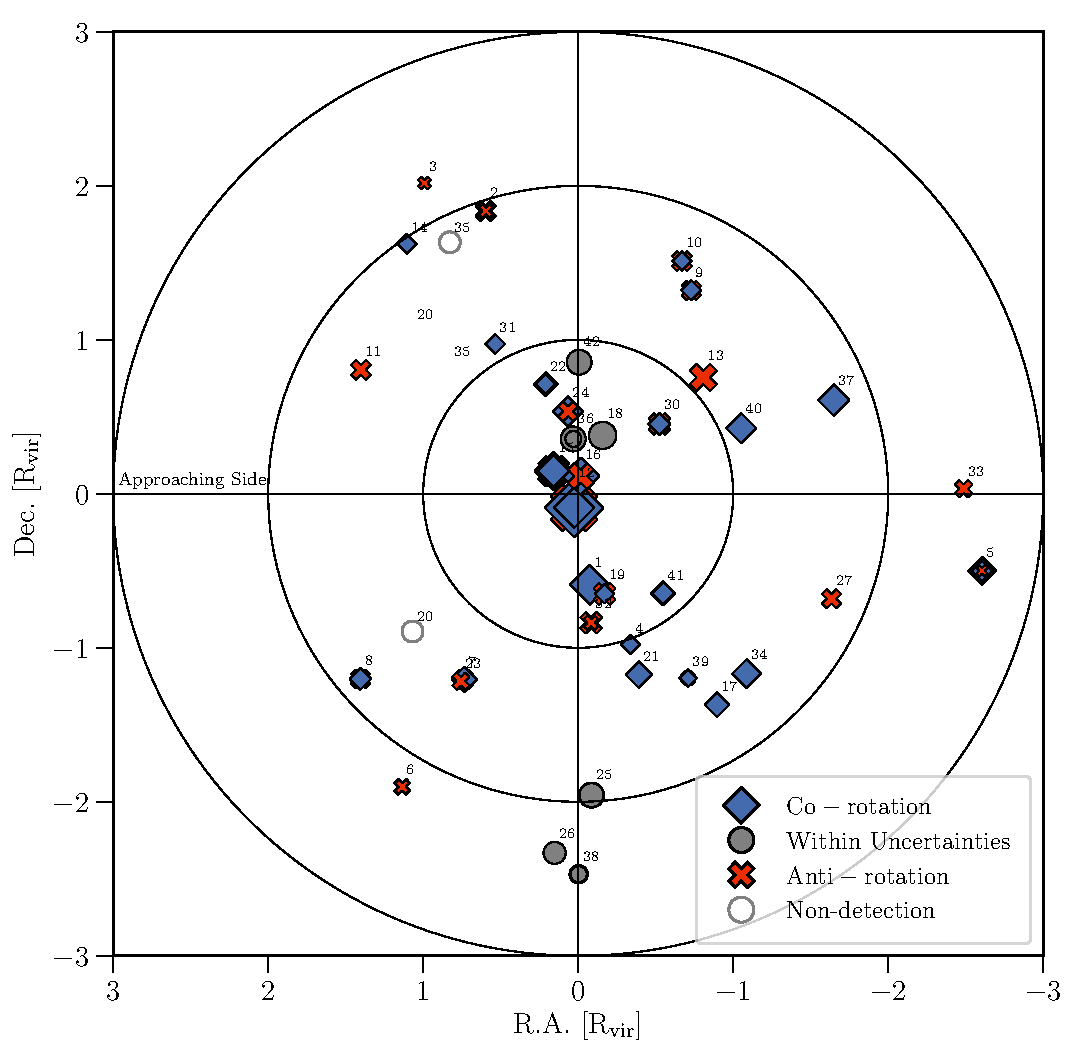
\includegraphics[width=0.95\textwidth]{SALTmap_velstrict_False_non_True_Lstar_0-100_minsep_False_inclim_00.pdf}
%        \caption{\small{A map of the locations of each absorber normalized with respect to the galaxy virial radius. The color and style of each point indicates the line-of-sight velocity compared to that of the rotation of the nearby galaxy. Blue diamonds indicate co-rotation, red crosses indicate anti-rotation, and grey circles indicate cases where either is possible due to a combination of orientation and velocity uncertainties. The size of each point is scaled to reflect the EW of the absorber. Concentric rings indicate distances of 1, 2, and 3 $R_{\rm vir}$. All galaxies are rotated to PA = 90 or 270, such that their major axis' are horizontal and their approaching side is on the left as indicated. The number identifiers correspond to the system number given in column (1) of Table \ref{model}.}}
%        \vspace{-5pt}
%        \label{full_map}
%\end{figure*}


%%\begin{figure*}
%%\centering
%%  \subfigure[]{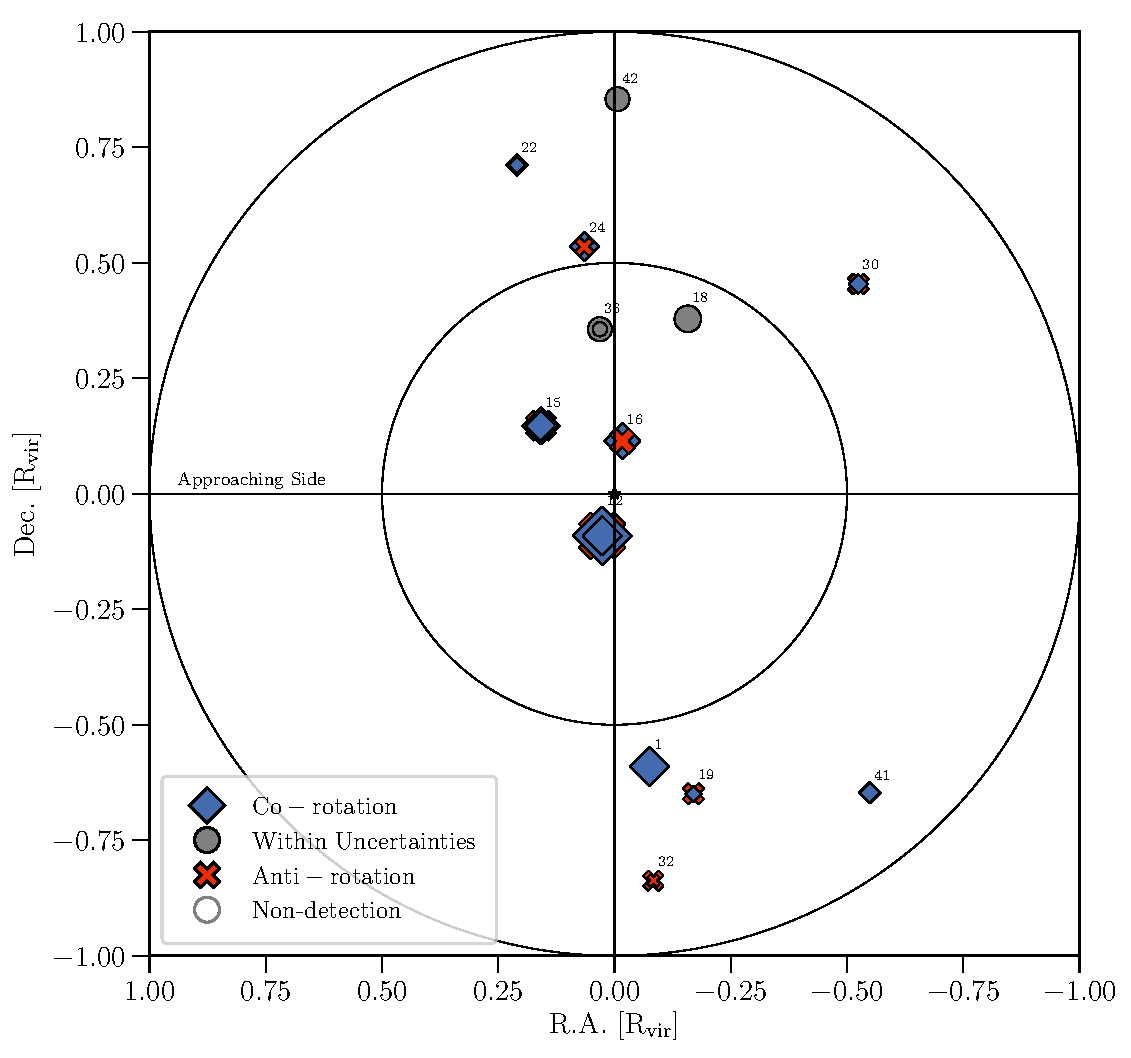
\includegraphics[width=0.5\linewidth]{SALTmap_velstrict_False_non_True_Lstar_0-100_minsep_False_zoom_10_inclim_00.pdf}}{\label{zoom_map}}
%%  \subfigure[]{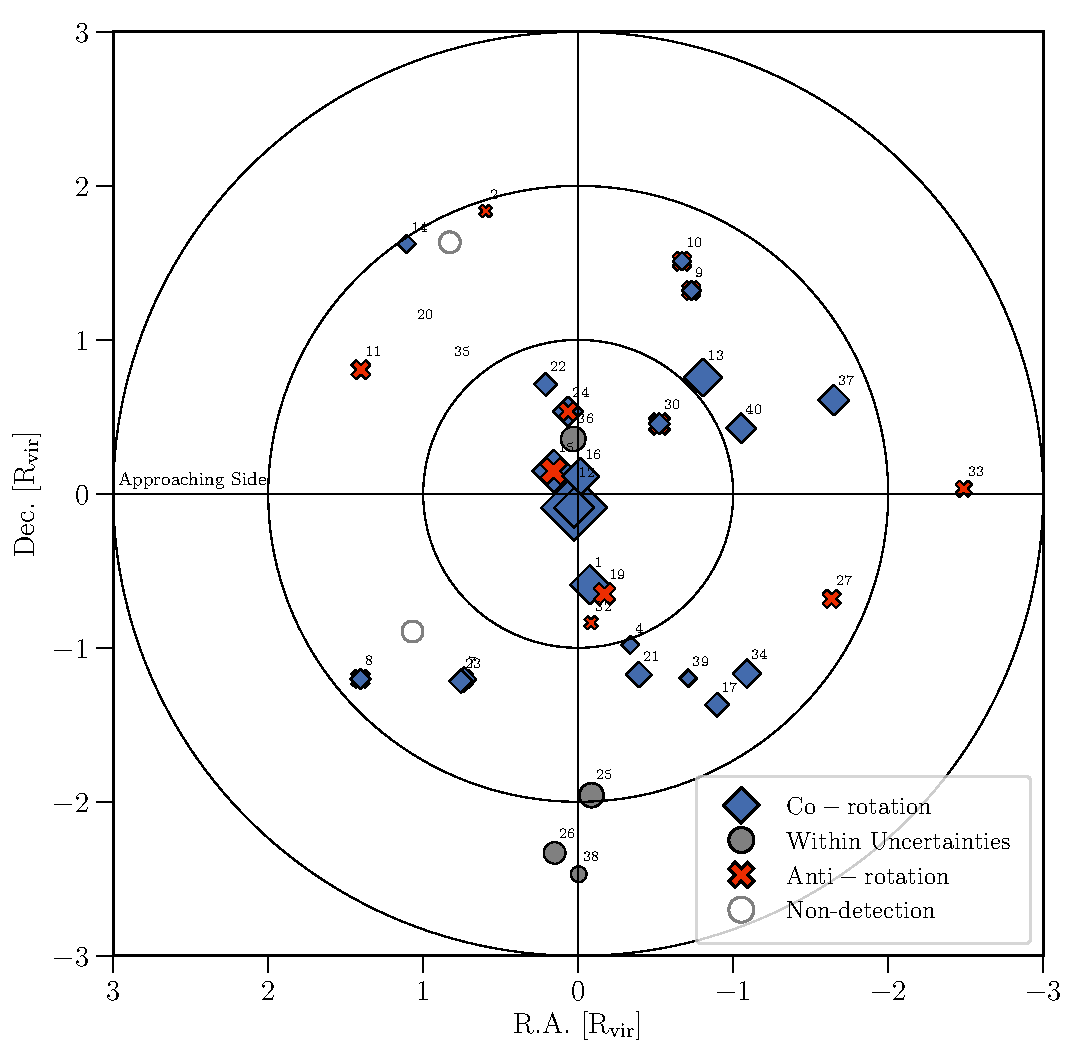
\includegraphics[width=0.48\linewidth]{SALTmap_NFW_model_velstrict_True_non_True_Lstar_0-100_minsep_False_inclim_00.pdf}\label{nfw_map}}
%%  \caption{\small{Maps of the locations of each absorber normalized with respect to the galaxy virial radius. \textbf{Left:} A zoom in showing only those systems within $1 R_{\rm vir}$. The color and style of each point indicates the line-of-sight velocity compared to that of the rotation of the nearby galaxy. \textbf{Right:} The color and style of each point indicates the NFW rotation model results for each absorber with a $v_{\rm Ly\alpha} \leq v_{\rm rot}$ constraint imposed. Concentric rings indicate distances of 1, 2, and 3 $R_{vir}$. \textbf{Both:} Blue diamonds indicate co-rotation, red crosses indicate anti-rotation, and grey circles indicate cases where either is possible due to a combination of orientation and velocity uncertainties. The size of each point is scaled to reflect the EW of the absorber. All galaxies are rotated to PA = 90 or 270, such that their major axis' are horizontal and their approaching side is on the left as indicated. The number identifiers correspond to the system number given in column (1) of Table \ref{model}.}}
%%\vspace{0pt}
%%\end{figure*}




\acknowledgements

D. M. F. thanks \textbf{A BUNCH OF PEOPLE}.This research has made use of the NASA/IPAC Extragalactic Database (NED) which is operated by the Jet Propulsion Laboratory, California Institute of Technology, under contract with the National Aeronautics and Space Administration. Based on observations with the NASA/ESA \textit{Hubble Space Telescope}, obtained at the Space Telescope Science Institute (STScI), which is operated by the Association of Universities for Research in Astronomy, Inc., under NASA contract NAS 5-26555. \textbf{SALT ACKNOWLEDGEMENT}. Spectra were retrieved from the Barbara A. Mikulski Archive for Space Telescopes (MAST) at STScI. Over the course of this study, D.M.F. and B.P.W. were supported by grant XXXX

%AST-1108913, awarded by the US National Science Foundation, and by NASA grants \textit{HST}-AR-12842.01-A, \textit{HST}-AR-13893.01-A, and \textit{HST}-GO-14240 (STScI). 

\facility{HST (COS), SALT (RSS)}
\clearpage

%\nocite{*}
%\bibliography{rotation_bib}
%\bibliography{/Users/frenchd/Research/bib}{}
\bibliography{/Users/frenchd/Research/inclination/git_inclination/bib}{}
\bibliographystyle{apj}

\clearpage

\appendix

\end{document}
